%!TEX root = ../username.tex
\chapter{Are Virtual Things Real?}
\section{Definitions}
At first glance, the question, an answer to the question "virtual things real?" appears trivial. Clearly, the pokemon in my handheld game are nothing more than a series of electromagnetic patterns. The same could be said of any sense-experience we have. 
Before we can investigate the claim "are virtual worlds real?", we must first establish what we mean by the claim. In his article \textit{The Virtual and the Real}, David Chalmers describes the term virtual as having several commonplace definitions. One common meaning of the term"virtual", claims the phrase"virtual X" means something along the lines of"as if X but not X" . On that reading, virtual reality is an unreal as-if reality, and virtual reality is no more reality than a virtual kitten is a kitten. \cite{ChalmersVR} While this definition is widely cited in dictionaries and other authoritative sources of definitions, it does not reflect the term’s contemporary definition. The advent of modern computer technology has resulted in a second widely used definition of the term"virtual". When used in discussions regarding computing, English speakers  tend to mean something along the lines of "a computer-based version of X" when talking about a"virtual X. Under this more contemporary description, virtual reality can be a sort of reality, just a virtual bank is a real bank (insofar as it fulfills all of the roles and functionalities we typically associate with an organization with the label of"bank"). 
For many readers, this recitation of definitions may appear pedantic. However, the dual definitions of the term"virtual" suggests that perhaps the opposition towards virtual realism is in part motivated by linguistics, just as proponents of the identity thesis in the philosophy of mind struggle with the inherent dualist bias in how English speakers and Western Philosophy think about these ideas. I will discuss this view of mine at greater length at later points in this paper, however for now I will merely say the first term should not be applied to descriptions of computer systems that instantiate via a combination of hardware and software an environment in which an agent can interact with entities described by software instructions. To apply the first term to these sorts of systems implies either confusion about the nature of these systems or an attempt to argue against virtual realism by begging the question. 
The second definition presented by Chalmers encompasses a wide array of systems and environments. These spaces range from the permanent and all-encompassing environment depicted in the 1999 science fiction movie \textit{The Matrix} to the ephemeral argumentation of the hit Android and iOS game, \textit{Pokemon Go}. In \textit{Matrix as Metaphysics}, Chalmers argues that"if we are in a Matrix, most of our ordinary beliefs (e.g. that there are tables) are true: if we discovered that we are in a Matrix, instead of saying that there are no tables, we should say instead that tables are computational objects made of bits". Chalmers describes this view as \textit{digitalism}, the claim that (1) Virtual objects really exist and are computational objects;
(2) Events in virtual worlds are largely computational events that really take place. (3) Experiences in virtual reality are non-illusory.
(4) Virtual experiences are as valuable as non-virtual experiences. In contrast to this view is the digital irrealist thesis, which claims that (1) Virtual objects do not really exist. (3) Experiences in virtual reality are illusory. \cite{ChalmersVR}. We shall be using two positions throughout this project as the two primary conflicting views on this topic. However, before we weigh the merits of virtual realism against its opposition, we must first have an account of what is real. This question has been an active battleground for philosophers since the field's inception, 2000 years ago. Most accounts of the real fall either into the dualist, idealist or materialist camps. Substance dualists (SD) hold that there exist two discrete types of substance, physical substance and mental substance.  Materialism is the claim that physical matter is the fundamental substance in the universe. This view is opposed by idealism, the claim that ideas or mental substance is fundamental material of reality. The idealist claims that the universe is purely mental, mentally constructed, or otherwise immaterial in nature. All of these positions are theoretically compatible with either virtual realism or virtual realism. However, each view comes with a series of caveats and ontological commitments which may be a deal breaker for many who hold said view. 




\subsection{Are virtual objects real?}
Virtual realism is unproblematic for the idealist, who asserts that all of reality is immaterial mental substance (in other words, ideas). However, Idealism is a highly outlandish view and difficult for many to wrap their heads around. Why ought we accept this view? The classical Western idealist position was first formalized by Bishop George Berkeley. Berkeley's rejection of the existence of physical substance is based upon the claim that we can perceive only our own ideas. Berkeley continues by arguing given that no inert substance (such as matter) can have ideas and since matter is an inert substance has sensible qualities, our understanding of matter is by definition contradictory in nature. Berkeley continues by claiming a denial of the claim "If sensible qualities are perceivable, then they must be ideas" in conjunction with his previous assertion that we can perceive only our own ideas implies a conception of matter that is epistemologically inaccessible and hence meaningless. \cite{berkeley2003a} We shall use a similar line of argumentation to justify a virtual realist conception of reality. Virtual objects are weapons, people, buildings and other entities within a virtual environment. These entities are instantiated within the memory of a digital computer by a data structure. Data structures consist of a series of values electromagnetically stored within the memory of the computer. When interpreted by a specific programming language, these values specify the number of bytes to allocate for a given instance or instances of a particular abstract object and specify a series of operations which can be applied to the data stored within the allocated memory. Every action in a given virtual world has a corresponding action within one or more data structure within the memory of the computer which is instancing said virtual world. These data structures can cause the computer to output electromagnetic data which can be transformed by other hardware into images, sounds and other forms of sense data. These electromagnetic emissions also enable it to communicate via wired or wireless connection with other computer systems. Humans and other conscious agents with the appropriate can perceive these electromagnetic emissions as sense-data. Clearly, data structures (via the hardware they are instantiated within) seem to have some level of causal powers. Computers fly jets, drive cars, perform surgery and drive multi-million user cross-continental worlds like EVE Online and World of Warcraft. Yet, books, movies and other forms of media also cause real world events. People clearly have strong emotional The virtual irrealist might claim that these data structures derive their causal power from the programmer who created them or the algorithm which generated them instead of arising from the data structures themselves. Under this view, data structures (and hence virtual objects) are ultimately patterns of interactions between different entities consisting of physical matter whose arrangement is set forth by the actions of a conscious entity. However, the same could be said of books and other other forms of media which the digital realist claims not to constitute real entities (or at least is not committed by definition to claiming). One direction for mitigating this problem is to bite the bullet and adapt a fictionalist stance, which holds that all fictional worlds are real in so much as we can say $\exists X$ where $X$ is some fictional entity within world $Y$. This line of reasoning is resembles modal realism, the position which claims that all possible worlds are as real as the actual world.\cite{lewis1986on} One proponent of this position is David Lewis. Lewis holds

One of the two major schools in Mahayana Buddhism, Yogacara is a form of Buddhistism noted for its denial of the existence of external objects \cite{siderits2007buddhism} . Literally translated, the term Yogacara means "the practice of yoga", this name reflects the school's origins in metaphysical speculation into the nature of yoga and mediation practices. Many advanced mediation practices involve focusing on ones awareness of purely mental entities, the connection between these expertises and the achievement of Enlightenment motivates the Yogacara's idealist understanding of the universe. Yogacaran metaphysics can be characterized by the term \textit{Cittamatra} (English: "consciousness only"), one of the school's other names. Yoagacarans believe that nothing exists besides mental things. This radical form of idealism seems highly counterintuitive and illogical. However, there are many persuasive arguments for this abnormal view. When somebody suffering from cataracts looks at the moon, they have the experience of seeing the moon as if it were covered in hairs. But clearly a hairy moon is no more real than a moon made out of cheese. Yet for the individual suffering from cataracts, their experience of a hairy moon is just as real as the experience of a desolate rocky moon was for the crew of Apollo eleven. So how do we account for what the person is seeing? Yogacaran philosopher Vasubandhu argues that the person with cataracts is aware of a mental image (deemed an impression) that manifests itself as an external object when there is no such thing outside of the mind. This view is motivated by representationalism, the notion that we "what we are directly aware of in waking memory sensory experience is not the external object, but rather a mental image that resembles the object and is caused by sense-object contact" \cite{siderits2007buddhism}.  \newline In contrast to the "impression only" idealism of the Yogacara, the representationalist viewpoint is compatible with the existence of external objects (i.e: a realist standpoint). Vasubandhu argues that the world is nothing but unreal impressions, analogous to the unreal hairs on the moon *seen* by the cataract sufferer.
 \newline
 Vasubandhu continues by denying the existence of spatial locations. Both realists and idealists like Vasubandhu describe experiences in terms of physical objects, but these experiences could also be explained in terms of images containing colors and shapes. Each of these color/shape images can be described as baring different relations to each other(left, right, etc) \cite{siderits2007buddhism}. This visual change will change over time, but an observer will eventually discover that certain visual features will reoccur periodically in a predicable manner. From these patterns, an agent can construct a phenomenal language that maps onto the all of the visual elements we typically describe in spatial terms. This language may be awkward, but it is the only means to describe these types of experiences in a manner that is amicable to both realists and idealists. This phenomenal language mirrors how computer systems describe and represent entities within a virtual space. Using this language, the realist can object to Vasubandhu's claim with the inter-subjective agreement \cite{siderits2007buddhism}. This argument centered around the fact that, barring special cases in which the experience is solely an impression (i.e: in the hairy moon example) agents seem to have remarkably similar sensory experiences. The realist claims that the different between these special impression-only experiences and *normal* sensory experience is that there is only a inter-subjective agreement in the latter scenario. In other words, the majority of observers are in agreement about the nature of the sensory experience and there are publicly accessible signifiers that can explain the minority's differences in sensory experience of the phenomena in question. From these facts, the realist claims, we can infer that normal sensory experience is independent of the observer's mind and therefore physical objects must exist. Another reply to Yogacaran idealism available to the realist is the argument from efficacy. This counterargument involves comparing sensory experiences which are known to be merely impressions with what are said to be normal sensory experiences. The normal sensory experiences will have clearly observable casual effects on the observer while the impressions have no lasting casual impact on the agent or their surroundings. \newline Vasubandhu counters these realist arguments with the phenomena of the \textit{pretas}, beings cursed to consume urine, blood and other vile things. Vasubandhu explains that karma causes the pretas to perceive an ordinary river as brimming with fowl liquids just as it causes the sinner to perceive the existence of demons and other guardians of hell. The pretas also present a counterexample to the inter-subjective agreement, the impression of a river of filth and demons is not merely the sensory-experience of a single entity, but rather the phenomenal  experience of everyone who has done evil in their past life.  




 Having shown shared karmic experience is an adequate substitute for physical substance for explaining the phenomena of intersubjective agreement.  Vasubandhu continues by arguing that spatio-temporal determinacy can be explained without positing the existence of physical objects. Vasubandhu cites dreams as an example of mere impressions the realist might claim exhibit spatio-temporal determinacy and efficacy. Dream entities clearly seem to have a discrete location at a given time within the dream world. Similarly, erotic dreams can have the same sorts of physical effects as an analogous intimate encounter outside of a dream state. \cite{siderits2007buddhism}.
 \newline
 
 For many, Vasubandhu's counterexamples will hardly seem sufficient to justify such an outlandish scheme as to propose the nonexistance of physical matter. After all, if we accept a Buddhist concept of karma, we are still left with two competing theories of experience: the impressions only explanation in terms of karmic seeds and the theory of karmic casual laws. \cite{siderits2007buddhism} Vasubandhu employs the \textit{principle of lightness}, a principle from Buddhist philosophy which states that "given two competing theories each of which is equally good at explaining and predicting the relevant phenomena, choose the lighter theory, that is, the theory which posits the least number of unobservable entities" \cite{siderits2007buddhism}. This principle motivates Vasubandhu's move to idealism, why should one posit the existence of material elements when the impressions-only theory has equal explanatory power? Realism introduces unnecessary complexity into our account of existence.  



  \section{Awareness and Virtual Reality}
A major factor when discussing the realism of a virtual environment is the agent or user's knowledge about said system. A user's sense of reality is highly dependent on their past experiences and subjective conception of reality. Just as the prisoners in Plato's  allegory of the cave believe the shadows on the wall to be real, an agent who was born and raised experiencing only the sense-data of digital environment like the one depicted in the movie \textit{The Matrix} will view sense-data from this machine as real, regardless of how unnatural or unreal it might appear to a human from "real world". Knowledge of whether one is a "brain in a vat" or within the "real world" is a major factor in determine of whether one doubts the reality of their experience. 
 \subsection{Materialism and VR}
Materialism holds that only finite physical substance embodies reality. For the materialist to accept virtual realism, they must adapt a strictly empiricist epistemological view, claiming sense-data is the sole source of justified true beliefs about the universe. For a materialist with this view, whatever they experience as the world around them is the world around them. A materialist born and raised in the Matrix would have no means (barring glitches in the Matrix) of deducing that she is experiencing sense-data that has been fed to her by a complex computer system. However, this view also is friendly to claims of virtual realism about contemporary VR technology. The output from a VR system is sense-data too. Interactions with objects in VR still have
\chapter{Quantifying the realness of virtual worlds }\label{text}
\section{Introduction}


Computer graphics have progressed immensely since the dawn of 3d computer graphics. Modern day computers are capable of rendering 3d models with with millions of polygons and employ complex shaders (computer programs that determine which colors and textures are used to draw the model) and other effects to create life-like images. However, realism in computer graphics is not merely a measure of the amount number of polygons or complexity of the shaders, physics engine or lighting effects. Small details like the uniqueness of terrain and objects, a lack of diversity in texture pattern and quality and other factors can have a significant impact on whether an environment appears realistic to a user. In this section, we shall survey and critique contemporary methods for quantitatively measuring realism in 3d computer worlds and posit our own measurement scheme. 


The term "realistic" compasses a wide array of subjective and objective qualities. One key factor in determining whether an experience in a 3d environment is realistic for a user is immersion. Authors in the field of digital communication and human-computer factors use the term “immersion” to describe a wide array of characteristics a digital space might have. Many authors use the term immersion to measure the ability of the system to "shut out:" or "pull" the user out of their awareness of physical reality. 
Slater and Wilbur (1997) note that an environment is more likely to feel immersive if it:
a) offers high fidelity simulations
through multiple sensory modalities, b) finely maps a user’s virtual bodily
actions to their physical body's counterparts, and c) removes the participant
from the external world through self-contained plots and narratives. 
These factors point to importance of sense of presence in making an immersive experience. However, other authors attempt to measure i through realistic graphics. Some researchers in this field attempt to quantify realism by taking snapshots of virtual environments and measuring aspects of the resulting images such as gradient variance, color variance and shadow
softness \cite{Wang:2011:RRP:2013879.2014089}. Others leverage qualitative data collected from user interviews to compare levels of realism between different virtual worlds and across hardware platforms. In this paper, we shall use the latter approach to measuring realness of virtual worlds. Our argument for the superiority of this methodology hinges on the fact that static screen-shots fail to account for the impact of animation, field of view, audio effects, type of control peripherals and other key aspects of user-experience on the immersiveness of an experience. A virtual environment's immersiveness is not merely a product of its graphics engine, physics engine and other software components but rather a composite of the proper application of software techniques and game design paired with a hardware system that well complements these software factors. As a result, it is improper to discuss the reality or immersive properties of
a piece of software independently of the hardware platform it is running on top of. 

\section{Emotion and immersion}
As described in introduction to this section, the realism of a virtual environment is a holistic measurement of the immersiveness of the player's experience within the game world. Games with inferior graphics systems but which feature a highly captivating story or game play mechanic are easier to lose oneself within then a bland game with state-of-the-art graphics. Central to a game or other form of simulation's ability to captivate a user is its capacity to invoke an emotional response in a user or player. Games with primitive graphics and game mechanics can still have powerful emotive power, Aerith's death in the 1997 JRPG (Japanese RPG) Final Fantasy VII still prompts strong emotional reactions, despite its primitive character models and linear gameplay in comparison with modern day games in the same genre. \cite{fig:FF7} 
\begin{figure}[ht!]
\centering
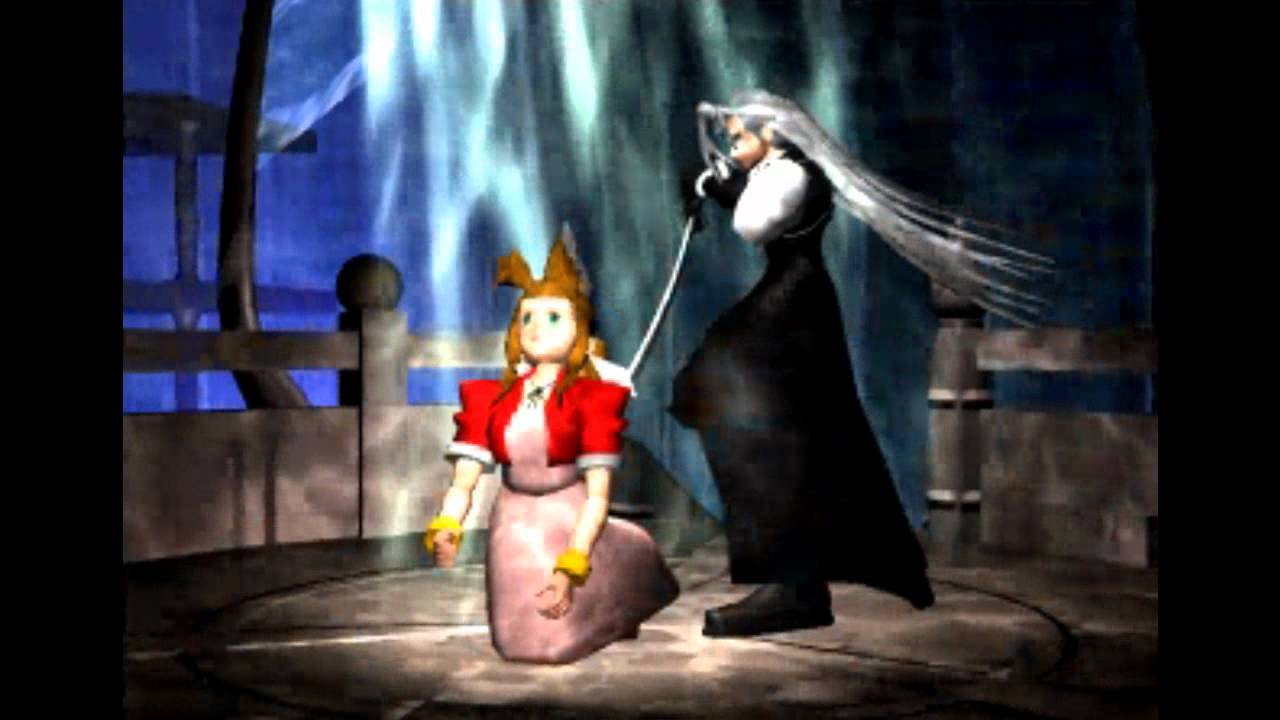
\includegraphics[width=90mm]{maxresdefault.jpg}
\caption{Final Fantasy 7 Aerith Death Cutscene \label{overflow}}
\label{fig:FF7}
\end{figure}
Clearly, the ability to invoke emotion is not something that can be measured using surface roughness or other such technical metrics. Storytelling is an essential aspect in creating an immersive experience. However, there are many games without plots that also offer a highly immersive experience for players. One such game is Minecraft, which offers players a 3d sandbox environment in which they must survive in a hostile world while building and exploring a procedurally generated voxel world containing caves mountains and countless other environments. This game features relatively primitive shaders and lighting effects and has a very minimal plot and few NPCs, yet the game still offers a highly immersive and addictive player experience. Players denote thousands of hours to building detailed and complex structures within the game world and express genuine stress and unease when faced with the in-game monsters, despite their unrealistic appearances. \cite{fig:MCmonster} 
\begin{figure}[ht!]
\centering
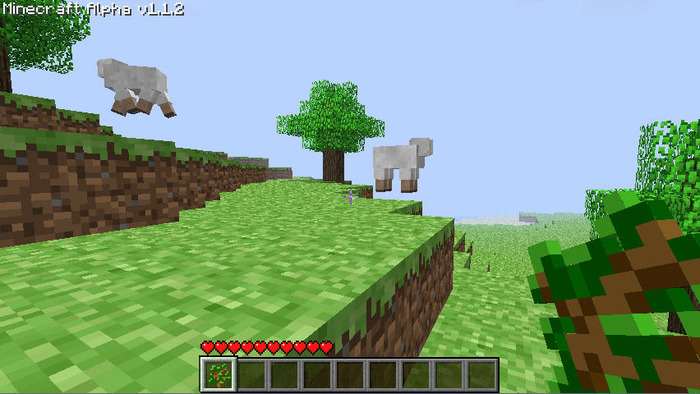
\includegraphics[width=90mm]{minecraft-32.jpg}
\caption{Minecraft Gameplay \label{overflow}}
\label{fig:Minecraft}
\end{figure}
\cite{fig:MCmonster} 
\begin{figure}[ht!]
\centering
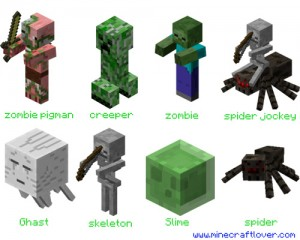
\includegraphics[width=90mm]{minecraft-spider-300x240.jpg}
\caption{Minecraft Hostile NPCs (source: http://www.minecraftlover.com) \label{overflow}}
\label{fig:MCmonster}
\end{figure}
A game's capacity to elicit an emotional response in the user is an essential and undeniable factor in its immersive qualities. We argue for  
\section[My new section]{An example of making a new section and giving it a short name}\label{sec:newsec}

The \ic{chapter} and \ic{subsection} commands work in exactly the same manner. Each new chapter must have \texttt{$\backslash$chapter[short name]\{chapter name\}} as its first line.

``Hey, wait a minute. What if I need to refer to that section? How can I do that?'' It's actually as simple as adding\verb+\label{labelname}+ at the end of the \ic{chapter} command like\texttt{$\backslash$section[My new section]\{An example of making a new section and giving it a short name\}$\backslash$label\{sec:newsec\}}. Now I can refer to Section \ref{sec:newsec} by typing \verb+\ref{sec:newsec}+. You can label just about anything and refer to the label to get an automatically generated number for the item. This means that you need to come up with a labeling scheme before you start writing and stick with it.

Some other things you'll need to be able to do include italicizing and bolding text and creating lists. These are also easy to accomplish. For example I can use \ic{emph} or \ic{textit} to italicize text. To italicize homework I would enter \verb|\emph{homework}| or \verb|\textit{homework}| to produce \textit{homework}. To obtain \textbf{bold} text you would use the \ic{textbf} command. And what about lists?

There are several kinds of lists\index{lists} (enumerated, itemized, and descriptive) and each has its own place and environment. An enumerated\index{lists!enumerated} list is good for outlining or ordered lists:

\begin{singlespace}
\begin{example}
\begin{enumerate}
\item First main idea
\begin{enumerate}
\item First subpoint
\item\label{enum:1b} Second subpoint
\end{enumerate}
\item Second main idea
\end{enumerate}
\end{example}
\end{singlespace}

The itemized\index{lists!itemized} list is good for unordered lists or bullet points:

\begin{singlespace}
\begin{example}
\begin{itemize}
\item Idea
\item Idea
\item Idea
\item Idea
\end{itemize}
\end{example}
\end{singlespace}

And the descriptive\index{lists!descriptive} list is good for definitions; however, \ip{amsthm} already has a definition environment, and you will most likely not need the description environment. In any event, here is an example:

\begin{singlespace}
\begin{example}
\begin{description}
\item[First item:] Idea
\item[Second item:] Idea
\item[Third item:] Idea
\end{description}
\end{example}
\end{singlespace}

Notice the use of brackets in the last example. The brackets are optional and the text in the brackets is used as the label for the item. You should also note that you can label an item for later reference see \ref{enum:1b}. There are several options for changing the format of the list environments and a package, \ip{paralist}, for customizing lists which are described in section 3.3 of \citet{mgbcr04}.

\section{Theorems, definitions, examples, oh my!}
The next thing you'll probably need to do is enter definitions, theorems, and examples. Below you will find some examples. On the left you will see the text typed into the document and on the right what it looks like when formatted. These examples are intended to give you a sense of what type of mathematical expressions \lt handles. You should look at Appendix~\ref{math} for a more complete discussion of entering mathematics. In the beginning you will not know all of the commands that you need to enter. Don't worry. Each of the suggested editors has a palette that shows you a picture of what you want and puts the correct commands into the document when you click the picture. As you look at these examples, keep it in mind that some of them use some user defined commands which can be found in \verb|styles/personal.tex|. Now lets look at Definition~\ref{def1} \ref{bdef1}, Theorem~\ref{introwatthm}, and equation~\ref{m.1diasumtwo}.

\begin{singlespace}
\begin{example}
\begin{defn}[One of Ramanujan's
 third order mock theta 
 functions]\label{def1}
 \begin{equation}\label{introf(q)} 
 f(q)=1+\sum_{y=1}^{\infty}
 \frac{q^{y^2}}{(1+q)^2(1+q^2)^2
 \cdots (1+q^y)^2}.
 \end{equation}\end{defn}
\end{example}
\end{singlespace}

\begin{singlespace}
\begin{example}
\begin{thm}[Watson's 
transformation of 
$f(q)$]\label{introwatthm}
\begin{equation}\label{introf}
\qrfac{q}{\infty}
\sum_{y=0}^{\infty} q^{y^2}
 \qrfac[-2]{- q}{y}=1+
 \sum_{y=1}^{\infty}
 \frac{(-1)^{y}
 4q^{(3/2)y^2+
 (1/2)y}}{(1+q^{y})}.
 \end{equation}\end{thm}
\end{example}
\end{singlespace}

This is a more complicated example which uses the \ic{substack} command to have multiple summation criteria.
\begin{singlespace}
\begin{example}
\begin{align}\label{m.1diasumtwo}
\left[NUM\right]_1^{(\fl)}(q;b;
\bvec{x})=&\ q\sum\limits_{
\substack{ 0\leq r,t 
\leq\fl-1}}
q^{r+t}\sum\limits_
 {\substack{{\lambda
 \vdash (r+t)}\\
  \lambda/1^r\in V_t\\
  \ell(\lambda)\leq \fl-1}}
  \mathrm{s}_{(b,\lambda)}
  (\bvec{x}).\end{align}
\end{example}
\end{singlespace}

Another thing that one might need to do is create piecewise definitions. This can be accomplished by using the \verb|cases| \index{cases@\verb+cases+} environment. This example also uses the \ic{intertext} command to put text between displayed equations.
\begin{singlespace}
\begin{example}\begin{subequations}\label{2c1BP}
\begin{alignat}{2}\label{2c1BPa} 
A_{y_1}:=&\begin{cases}
 1 &\text{for $y_1=0$},\\
\frac{-1)^{y_1}
4q^{y_1}q^{\binom{y_1}{2}}}
{\qrfac{q}{2y_1}(1+q^{y_1})}
&\text{for $y_1>0$}\end{cases}\\
\intertext{and} B_{y_1}:=&
\qrfac[-1]{-q}{y_1}\qrfac[-1]
{-q}{y_1}=\qrfac[-2]{-q}{y_1}
&.\label{2c1BPb}\end{alignat}
\end{subequations}
\end{example}
\end{singlespace}

Finally, if you need to incorporate examples into your thesis you can do it using the example environment, as seen in Example~\ref{ex:ex}.
\begin{singlespace}
\begin{example}
\begin{ex}[An example example]
\label{ex:ex}
This is an example of including an
 example. Kind of silly isn't it.
 \end{ex}
\end{example}
\end{singlespace}

\section{Putting code in the main body of the thesis}
There is one last textual item which Computer Science majors and probably some Mathematics majors will need to incorporate, pseudocode\index{pseudocode}. To do this I would suggest using the \ic{lstlisting} environment. Below is an example set up for the \ip{listings} package. You could put your modifications to this set up into the \texttt{personal.tex} file in the \texttt{styles} folder. Documentation on the \ip{listings} package can be found in the \texttt{doc} folder with the documentation for the other packages.
\lstset{
               language =Pascal, % pick a language style
               emph={return,natural, numbers, integers, increasing},
               emphstyle={\bfseries},% choose other keywords and a format
               linewidth=.95\textwidth, breaklines=true, commentstyle=\textit,
               stringstyle=\upshape, showspaces=false, numbers=left,
               numberstyle=\tiny, basicstyle=\small, xleftmargin=30pt,
               breakautoindent=true, captionpos=b
               }
{\small\begin{singlespace}
\begin{verbatim}
\lstset{
        language =Pascal, % pick a language style
        emph={return,natural, numbers, integers, increasing},
        emphstyle={\bfseries},% choose other keywords and a format
        linewidth=.95{\textwidth}, breaklines=true,commentstyle=\textit,
        stringstyle=\upshape,showspaces=false,numbers=left,
        numberstyle=\tiny,basicstyle=\small,xleftmargin=30pt,
        breakautoindent=true,captionpos=b
        }
\end{verbatim}
\end{singlespace}}

The listing in Listing~\ref{largesteven} gives an algorithm for finding the largest even integer in a given list of $n$ integers. I have used the \texttt{mathescape}\index{listings!mathescape} option to be able to incorporate mathematics in the listing. The actual code put in the thesis is given first and the formatted output follows.

{\small\begin{singlespace}
\begin{verbatim}
\begin{lstlisting}[mathescape, caption= Find the location 
of the largest even integer in a list,label=largesteven]
procedure $largestevenlocation$($a_1, a_2, \ldots, a_n$: integers)
$k$:=0
$largest$:=-$\infty$
for $i$:=1 to $n$
  if ($a_i$ is even and $a_i>largest$) then
  begin
    $k$:=$i$
    $largest$:=$a_i$
  end
end
return $k$
\end{lstlisting}
\end{verbatim}
\end{singlespace}
}
\begin{singlespace}
\begin{lstlisting}[mathescape, caption= Find the location
 of the largest even integer in a list,label=largesteven]
procedure $largestevenlocation$($a_1, a_2, \ldots, a_n$: integers)
$k$:=0
$largest$:=-$\infty$
for $i$:=1 to $n$
  if ($a_i$ is even and $a_i>largest$) then
  begin
    $k$:=$i$
    $largest$:=$a_i$
  end
end
return $k$
\end{lstlisting}
\end{singlespace}
The code in Listing~\ref{quartsearch} is an improvement on Binary search. The algorithm reduces the size of the search by a factor of four at each iteration. It provides another example of using the \ic{lstlisting} environment.
\begin{singlespace}\small
\begin{verbatim}
\begin{lstlisting}[mathescape,caption=Quartary search,
label=quartsearch]
procedure $quartarysearch$($x$: integer, $a_1, a_2,
 \ldots, a_n$: increasing integers)
$i$:=$1$
$j$:=$n$
while $i<j-2$
begin
  $l:=\lfloor(i+j)/4\rfloor$
  $m:=\lfloor(i+j)/2\rfloor$
  $u:=\lfloor3(i+j)/4\rfloor$
  if $x>a_m$ then
    if $x\leq a_u$ then
    begin
      $i:=m+1$
      $j:=u$
    end
    else
     $i:=u+1$
  else if $x>a_l$ then
    begin
      $i:=l+1$
      $j:=m$
    end
    else $j:=l$
end
if $x=a_i$ then $location:= i$
else if $x=a_j$ then $location:= j$
else if $x=a_{\lfloor(i+j)/2\rfloor}$ then
 $location:= \lfloor(i+j)/2\rfloor$
else $location:= 0$
return $location$
\end{lstlisting}
\end{verbatim}
\end{singlespace}
\begin{singlespace}
\begin{lstlisting}[mathescape,caption=Quartary search,label=quartsearch]
procedure $quartarysearch$($x$: integer, $a_1, a_2, \ldots, a_n$: increasing integers)
$i$:=$1$
$j$:=$n$
while $i<j-2$
begin
  $l:=\lfloor(i+j)/4\rfloor$
  $m:=\lfloor(i+j)/2\rfloor$
  $u:=\lfloor3(i+j)/4\rfloor$
  if $x>a_m$ then
    if $x\leq a_u$ then
    begin
      $i:=m+1$
      $j:=u$
    end
    else
     $i:=u+1$
  else if $x>a_l$ then
    begin
      $i:=l+1$
      $j:=m$
    end
    else $j:=l$
end
if $x=a_i$ then $location:= i$
else if $x=a_j$ then $location:= j$
else if $x=a_{\lfloor(i+j)/2\rfloor}$ then $location:= \lfloor(i+j)/2\rfloor$
else $location:= 0$
return $location$
\end{lstlisting}
\end{singlespace}

\section{What is in \texttt{username.tex}}
Before we move on let's talk a little bit about what is at the beginning of \verb|username.tex|. The file starts with 
\verb|\documentclass{woosterthesis}|, which must be at the beginning of every IS. In the brackets are options for the woosterthesis class. The options are the same as for the \verb|book| class with some additional options  \verb|abstractonly|\index{woosterthesis options!abstractonly}, \verb|alltt|\index{woosterthesis options!alltt},  \verb|blacklinks|\index{woosterthesis options!blacklinks}, \verb|code|\index{woosterthesis options!code}, \verb|dropcaps|\index{woosterthesis options!dropcaps}, \verb|euler|\index{woosterthesis options!euler}, \verb|guass|\index{woosterthesis options!guass}, 
\verb|index|\index{woosterthesis options!index}, \verb|kaukecopyright|\index{woosterthesis options!kaukecopyright}, \verb|palatino|\index{woosterthesis options!palatino}, \verb|picins|\index{woosterthesis options!picins}, \verb|verbatim|\index{woosterthesis options!verbatim}, and \verb|xetex|\index{woosterthesis options!xetex}. The \verb|kaukecopyright| option will put the arch symbol with the word mark on the copyright page. The \verb|blacklinks| option will make the hyperlinks in the PDF version of the thesis black and suitable for printing; normally the links are colored to provide visual clues to the reader.  The \verb|code| option will use \ip{listings} style to format program code examples.  The \verb|abstractonly| option will allow you to print just the Abstract. The \verb|palatino| option will use the \ip{pxfonts} package which uses the Palatino fonts. The \verb|picins| option will use the \ip{floatflt} package to allow text to wrap around images. \verb|index| will allow the \ip{makeidx} package to be loaded so that if you have index entries they will be added to an index (this reqires additional steps). \verb|dropcaps| loads the \ip{letterine} package for doing dropped capitals and \verb|alltt| loads the \ip{alltt} for using typewriter type in various ways. \verb|verbatim| allows one to set verbatim what is entered. \verb|euler| and \verb|guass| load the \ip{woofncychap} package with the named option which will change the look of chapter headings. Finally \verb|xetex| will allow you to use the \ifthenelse{\boolean{xetex}}{\XeTeX\ }{XeTeX} extension of \TeX{} for easy use of system fonts. Adding or deleting options from the comma separated list will change the appearance of the document and some options should only be used after consulting your advisor. Now let's move on to some other things that you'll need to deal with: figures, pictures, and tables.
